\documentclass[byrevtex,amssymb,aps,pra,floatfix,letterpaper]{revtex4}
\usepackage{graphicx}
\usepackage{hyperref}
\usepackage{verbatim}
\usepackage{amsmath}
\bibliographystyle{apsrev}
\date{\today}
\pagestyle{plain}
\newcommand{\degree}[0]{$^\circ$}

\begin{document}

\title{Experiment 2: Kinetics of a reversible, first-order, consecutive reaction}

\date{\today}

\maketitle

\section{Introduction}

The majority of chemical reactions do not take place at a single collision but rather have a reaction mechanism, which involves several elementary reaction steps. Thus the reaction may not follow a simple first- or
second-order rate law. When the rate law is inconsistent with the stoichiometry of the chemical equation, the reaction cannot be elementary. An example is the oxidation of the formate ion by permangate in water, which has been observed to be second-order experimentally:

\begin{align}
\label{eq1}
& 2\textnormal{MnO}^-_4 + 3\textnormal{HCO}^-_2 \rightarrow 2\textnormal{MnO}_2 + \textnormal{HCO}^{2-}_3 + \textnormal{H}_2\textnormal{O}\\
\notag
& -\frac{d\left[\textnormal{HCO}^-_2\right]}{dt} = k_2\left[\textnormal{HCO}_2^-\right]\left[\textnormal{MnO}_4^-\right]
\end{align}

\noindent
The stoichiometry immediately establishes that the reaction must be more complex than a single bimolecular reaction step. Although reactions consisting solely of a simple bimolecular encounter process will give second-order kinetics, the converse is not necessarily true.

The differential form of the rate law is usually much easier to write than the corresponding integrated rate law. There is no general method of solving complex differential rate equations, since each case usually requires a specific treatment. In many problems it is not possible to find analytic solutions and in such cases only numerical methods can be applied. Special methods exist, for example, for the following three important cases \cite{ATKINS1,SILBEY,COX}:

\begin{enumerate}
\item Reversible reactions, or reactions proceeding towards equilibrium, wherein measurable concentrations of reactants remain.

\item Concurrent or side reactions which control product distribution where more than one process is available to a reactant.

\item Consecutive reactions where the initial products are reactants for subsequent reactions.
\end{enumerate}

\noindent
In this laboratory excercise kinetics of the oxidation of tripeptide gluthatione-$\gamma$-L-glutamyl-L-cysteinylglycine (GSH; see Fig. \ref{eq1}) by Cr(VI) is studied at $pH$ 6, which results in formation of glutathionyl disulfide (``oxidized GSH'', GSSG; see Fig. \ref{eq2}). The overall reaction mechanism for the reaction has been determined as:

\begin{equation}
\label{eq2}
2\textnormal{CrO}_4^{2-} + 6\textnormal{GSH} + 10\textnormal{H}^+ \rightarrow 2\textnormal{Cr}^{3+} + 3\textnormal{GSSG} + 8\textnormal{H}_2\textnormal{O}
\end{equation}

\begin{figure}[!htp]
\begin{center}
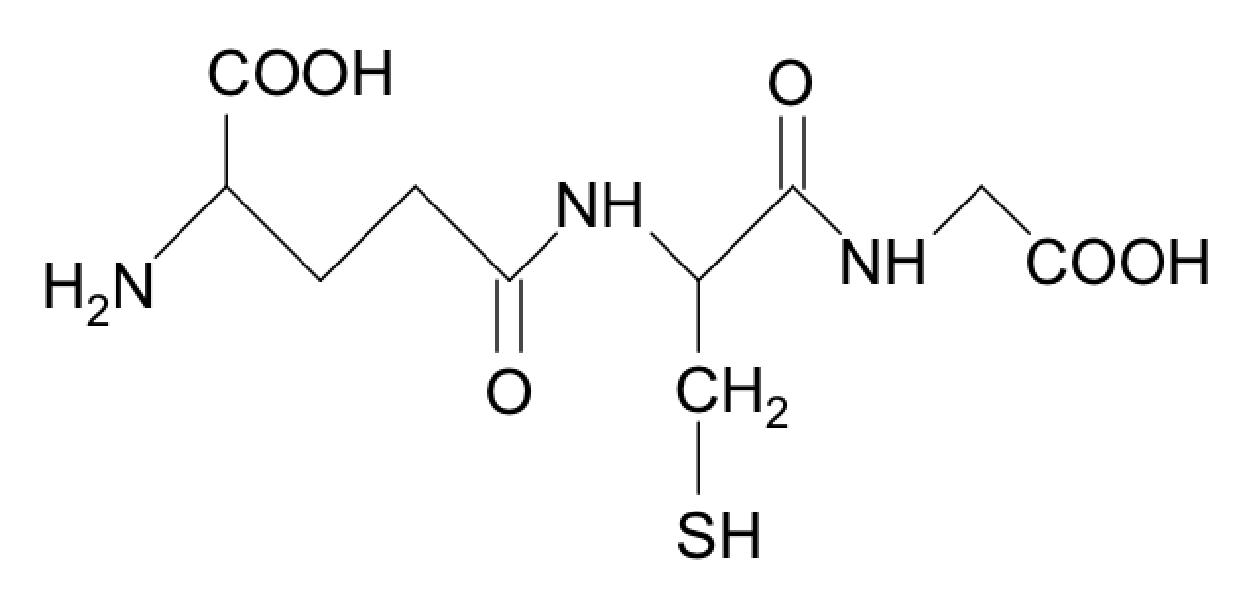
\includegraphics[scale=0.3]{fig1}
\caption{A two dimensional structure of GSH is shown (``reduced GSH'').}
\label{fig1}
\end{center}
\end{figure}

\begin{figure}[!htp]
\begin{center}
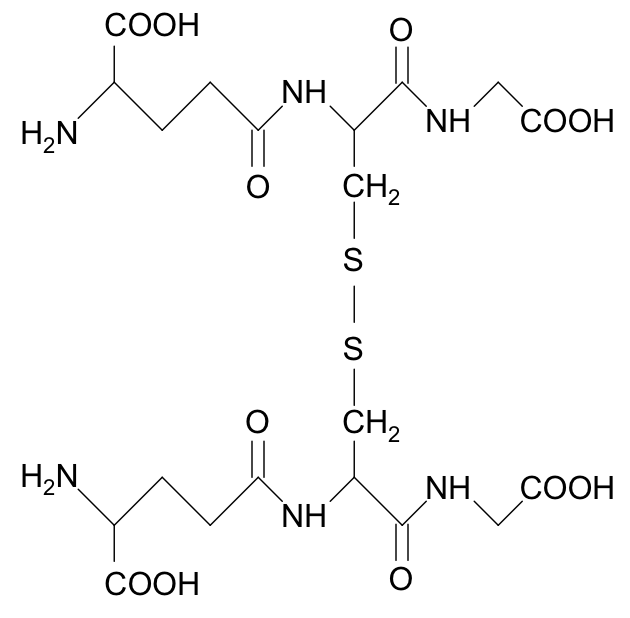
\includegraphics[scale=0.3]{fig2}
\caption{A two dimensional structure of GSSG is shown (``oxidized GSH'').}
\label{fig2}
\end{center}
\end{figure}

\noindent
This reaction is believed to partly account for the toxicity and carcinogenicity of Cr(VI). GSH and GSSG function as a redox couple, both in intracellular and plasma environments. GSH provides an important defense mechanism against certain toxic compounds, such as some drugs and carcinogens. If the levels of GSH in a tissue such as liver are lowered, then that tissue have been shown to be more susceptible to injury by various chemicals that would normally be conjugated to GSH.

The reaction consists of two consecutive and one reversible step (i.e, categories 1 and 3 above), which can be written as:

\begin{eqnarray}
\label{eq3}
& & \textnormal{(I)\phantom{I} }\textnormal{CrO}_4^{-2} + \textnormal{GSH} \rightleftharpoons \textnormal{CrO}_4^{2-}\textnormal{-- GSH}\\
\nonumber
& & \textnormal{(II) } \textnormal{CrO}_4^{2-}\textnormal{-- GSH} + \textnormal{GSH} \rightarrow \textnormal{GSSG} + \textnormal{Cr}^{3+}
\end{eqnarray}

\noindent
With excess concentrations of GSH and H$^+$, all three reaction steps (i.e., forward and backward reactions in (I) and forward reaction in (II)) follow effectively first order kinetics. High-order reactions that behave like first order reactions in presence of excess concentrations of the reactants are called pseudo first order reactions.

For more information on kinetics, see Refs. \cite{ATKINS1,SILBEY,CHANG,COX}.

\section{Kinetics}

In this work excess concentrations of GSH and H$^+$ are present and thus all of the reactions follow first order kinetics (i.e., the isolation method). As will be discussed later on, the concentrations of Cr ions are monitored in this experiment and therefore the rate equations are written in terms of their concentrations (not GSH or GSSG). When we denote $r = \left[\textnormal{CrO}_4^{2-}\right]$, $i = \left[\textnormal{CrO}_4^{2-}\textnormal{-- GSH}\right]$, and $p = \left[\textnormal{Cr}^{3+}\right]$, the reaction mechanism can be written as:

\begin{equation}
\label{eq4}
r \mathop\rightleftharpoons\limits_{k_3}^{k_1} i \mathop\rightarrow\limits^{k_2} p
\end{equation}

\noindent
The empirical differential rate equations for this reaction can be written as:

\begin{eqnarray}
\label{eq5}
& & \frac{dr(t)}{dt} = -k_1r(t) + k_3i(t)\\
\nonumber
& & \frac{di(t)}{dt} = k_1r(t) - (k_3 + k_2)i(t)\\
\nonumber
& & \frac{dp(t)}{dt} = k_2i(t)
\end{eqnarray}

\noindent
where functions $r(t)$, $i(t)$ and $p(t)$ are functions that determine concentrations of components $r$, $i$ and $p$ at given time $t$. In mathematical terms Eq. (\ref{eq5}) represents three coupled ordinary differential equations. Obtaining their analytic solution is quite laborious and here, instead of solving the problem with a pen and paper, we demonstrate the use of a modern symbolic algebra package (e.g., Maxima \cite{MAXIMA}). The following maxima program will compute the unknown functions $r$, $i$ and $p$, which satisfy Eq. (\ref{eq5}):\\

\verbatiminput{maxima/diffeq.mac}

\noindent
The above program is available as a Maxima batch file on the laboratory course web page. The program can be run under wxMaxima graphical user interface by choosing ``File $\rightarrow$ Batch file'' (see the general section in the laboratory manual for details). Even though programs like Maxima can perform symbolic calculations, \textit{the results should always be double checked with a pen and paper}! The relevant part of the output resides at the very end and looks like:

\begin{eqnarray}
\label{eq6}
& & [r\left( t\right) =\frac{a\,r_0\,{e}^{-l_2\,t}}{a+1}+\frac{r_0\,{e}^{-l_1\,t}}{a+1},\\
\label{eq7}
& & i\left( t\right) =-\frac{a\,l_2\,r_0\,{e}^{-l_2\,t}}{a\,l_2+l_2-a\,l_1-l_1}-\frac{l_1\,r_0\,{e}^{-l_2\,t}}{a\,l_2+l_2-a\,l_1-l_1}+\frac{a\,l_2\,r_0\,{e}^{-l_1\,t}}{a\,l_2+l_2-a\,l_1-l_1}+\frac{l_1\,r_0\,{e}^{-l_1\,t}}{a\,l_2+l_2-a\,l_1-l_1},\\
\label{eq8}
& & p\left( t\right) =\frac{l_1\,r_0\,{e}^{-l_2\,t}}{l_2-l_1}-\frac{l_2\,r_0\,{e}^{-l_1\,t}}{l_2-l_1}+r_0]
\end{eqnarray}

\noindent
where subscripts have been inserted for clarity and $r_0$ denotes the initial concentration of the reactant $r$. Note that the initial concentrations of $i$ and $p$ were assumed to be zero. The following notations were used in order to obtain the simplified expressions:

\begin{equation}
\label{eq9}
k_1 = \frac{a\times l_2 + l_1}{a + 1}\textnormal{, }k_2 = \frac{l_1\times l_2}{k_1}\textnormal{, }k_3 = l_1 + l_2 - k_1 - k_2
\end{equation}

\noindent
which relate the variables in Eqs. (\ref{eq6}, \ref{eq7}, \ref{eq8}) to rate constants $k_1$, $k_2$ and $k_3$. Thus variables $a$, $l_1$, and $l_2$ determine $k_1$, $k_2$, and $k_3$. Given $k_1$, $k_2$, $k_3$, and $r_0$, Eqs. (\ref{eq6}, \ref{eq7}) predict time dependent the behavior of concentrations for species $r$ (i.e., CrO$_4^ {2-}$), $i$ (i.e., CrO$_4^{2-}$--GSH), and $p$ (i.e., Cr$^{3+}$). Eqs. (\ref{eq6}, \ref{eq7}) can be simplified as follows:

\begin{eqnarray}
\label{eq67a}
& & r(t) \propto e^{-l_1t} + a e^{-l_2t}\\
& & i(t) \propto e^{-l_1t} - e^{-l_2t}
\end{eqnarray}

\noindent
Note that if we don't know the prefactors for these expressions, $i(t)$ alone cannot be used to determine $a$. In this experiment both $r(t)$ and $i(t)$ will be analyzed simultaneously and this will give $l_1, l_2$ and $a$, and finally $k_1, k_2$ and $k_3$.

In this work we will be mainly interested in Eqs. (\ref{eq6}) and (\ref{eq7}). Both functions $r(t)$ and $i(t)$ consist essentially of a sum of two exponential functions. In Eq. (\ref{eq6}) both of the terms have the same sign but different weight and therefore function $r(t)$ exhibits bi-exponential decay as shown in Fig. \ref{fig3}. In Eq. (\ref{eq7}), however, the exponentials have opposite signs, which results in both raise and decay behavior as demonstrated in Fig. \ref{fig4}.

\begin{figure}[!htp]
\begin{center}
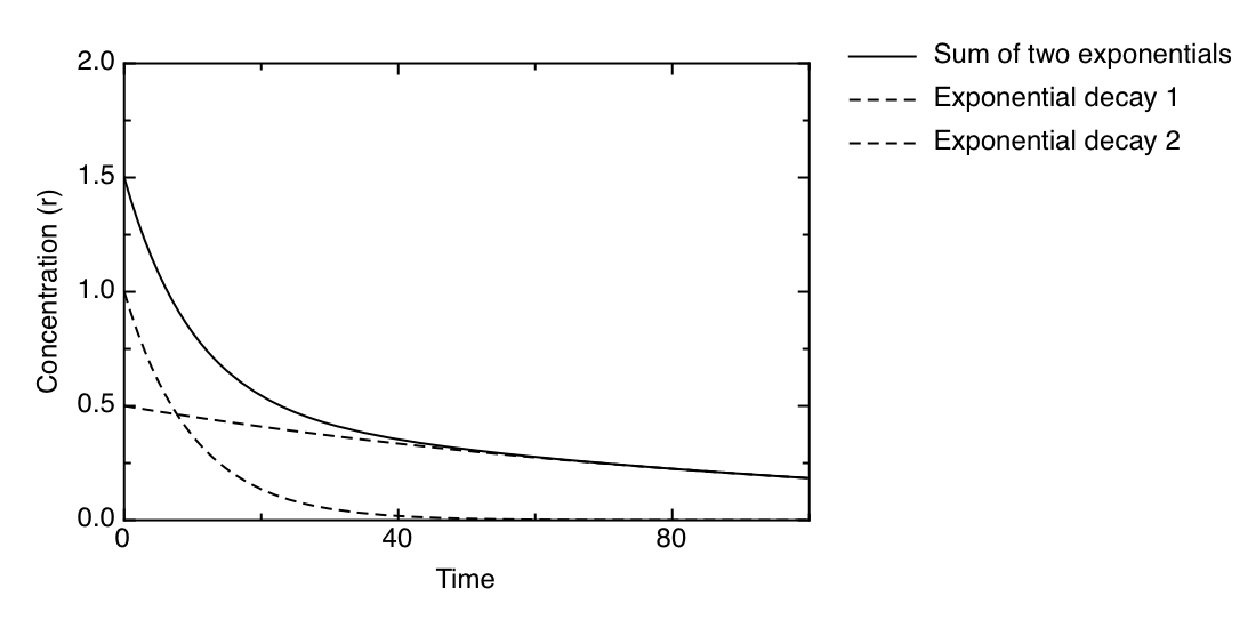
\includegraphics[scale=0.5]{fig3}
\caption{An example of a bi-exponential decay consisting of two exponent functions (see Eq. (\ref{eq6})) with the same sign. The exponential functions have different decay rates and weights. As an example, the following (random) values were used $l_1 = 0.1$, $l_2 = 0.01$, $a = 0.5$, and $r_0 = 1.5$.}
\label{fig3}
\end{center}
\end{figure}

\begin{figure}[!htp]
\begin{center}
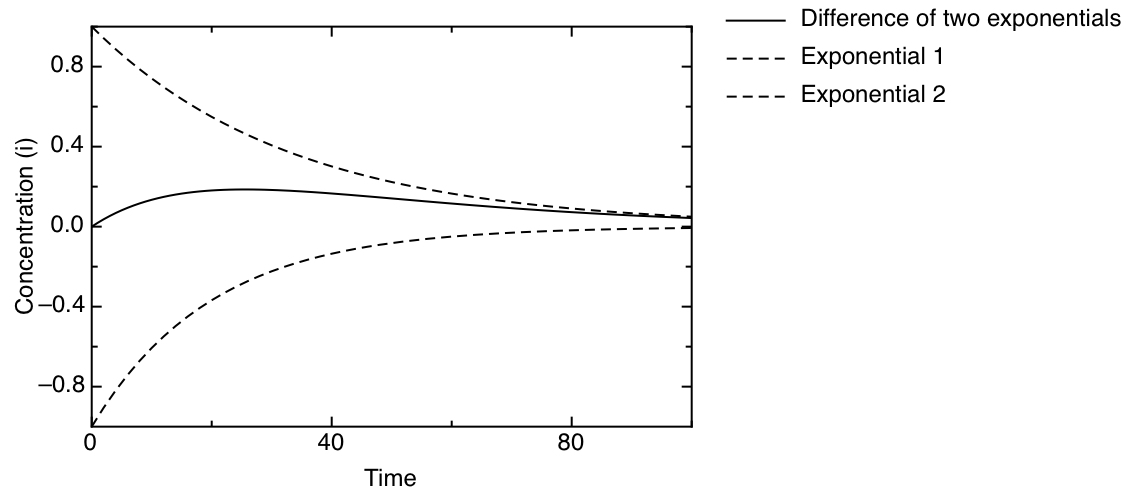
\includegraphics[scale=0.5]{fig4}
\caption{An example of raise and decay periods resulting from a difference of two exponent functions. The following values in Eq. (\ref{eq7}) were used: $l_1 = 5 \times 10^{-2}$, $l_2 = 2 \times 10^{-2}$, and the pre-factor containing variables $r_0$, $a$ etc. was set to one.}
\label{fig4}
\end{center}
\end{figure}

\section{Kinetics with UV/VIS spectroscopy}

Kinetics of a given species (i.e., its time dependent concentration) can be measured by monitoring light absorption at a given wavelength as a function of time. The fundamental equation in UV/VIS spectroscopy is the Beer-Lambert law:

\begin{equation}
\label{eq10}
A = \epsilon c L
\end{equation}

\noindent
where $A$ denotes absorbance (dimensionless), $\epsilon$ is the molar absorption coefficient at specified wavelength (usually specified as a subscript; mol$^{-1}$ L cm$^{-1}$), $c$ is the concentration of the absorbing species (mol L$^{-1}$), and $L$ is the sample length (cm). The molar absorption coefficient depends on the wavelength, the absorbing species, solvent etc. and hence it would have to be determined separately by using a calibration solution with a known concentration.  In this experiment, only relative concentrations are needed (i.e., $A \propto c$) and hence no additional calibration measurements for determining $\epsilon$ are made.

Another frequently occurring problem is that multiple species have overlapping absorptions in a UV/VIS spectrum. If only one wavelength is monitored, like in typical UV/VIS kinetics runs, it is not possible to distinguish the absorbing species from each other. This often complicates kinetics studies that employ UV/VIS spectroscopy as a tool
for monitoring concentrations. Two different cases of overlap can occur: (I) species overlap but only concentration of one of the components change over time or (II) concentrations of all species change. In the second case, UV/VIS spectroscopy can only be applied when the spectral composition of the absorption is known exactly. In the first case, however, the other species merely provide a constant baseline in the spectrum, which can be subtracted from the experimental data.

\section{Experimental method}

The time dependence of the Cr(VI) concentration can be followed by monitoring its absorbance at 370 nm and the CrO$_4^{2-}$--GSH intermediate at 430 nm. The reaction rate is highly dependent on pH as well as the buffer composition and concentration. Hence, the reaction conditions have to be chosen carefully for the system to exhibit well-resolved kinetics in a suitable time-scale.\\

\noindent
\underline{Safety precautions:} \textit{Protective gloves must be worn when working with chromium compounds. After the experiment, dispose all chromium-containing solutions in a heavy-metal waste container.}\\

\noindent
The following aqueous stock solutions are provided:\\

\noindent
\begin{tabular}{l@{\extracolsep{2cm}}l}
0.40 M K$_2$HPO$_4$   &     The buffer\\
5.0 $\times$ 10$^{-3}$ M HCl &    For adjusting the pH\\
1 M HCl and 1 M NaOH & To trim the pH\\
1.6 $\times$ 10$^{-3}$ M K$_2$Cr$_2$O$_7$ & The oxidant\\
\end{tabular}\\

\noindent
The following water solution must be prepared:\\

\noindent
\begin{tabular}{l@{\extracolsep{2.9cm}}l}
8.0 $\times$ 10$^{-3}$ M GSH & The reductant. Molecular weight of GSH (glutathione, \\
 & reduced) is 307.32 g mol$^{-1}$.\\
\end{tabular}\\

\noindent
Note that GSH solutions undergo slow oxidative degradation in air and therefore they should not be stored for long periods of time. Prepare the solution in a 50 mL volumetric flask on the day of the experiment.\\

\noindent
Small volumes ($<$ 10 mL) of the first three solutions are needed; 20 mL of the GSH solution is required.\\

\noindent
\underline{The procedure}:\\

\noindent
\begin{enumerate}
\item Pipet 20 mL of the GSH solution into a small beaker or flask where a pH electrode can be inserted. Pipet 4 mL of the K$_2$HPO$_4$ buffer and 6 mL of the 5.0 $\times$ 10$^{-3}$ M HCl solution into that vessel. Mix thoroughly and measure the pH. Add drop by drop a sufficient amount of 1 M HCl (or NaOH) to bring the pH to 6.0.

\item Turn on the Hewlett-Packard Diode Array UV/VIS spectrometer (at the bottom). Wait for a minute and then turn on the computer. After the computer has started, press Ctrl-Alt-Del simultaneously, enter the password: ChemUVVis . Click START, PROGRAM, HPUV, and then chose INSTRUMENT 1 ONLINE. Press CANCEL when the program asks for login.

\item In the menu at the top of the screen, check that MODE is set for KINETICS. Click on SETUP (Time \& Calculation). Set the wavelength at 430 nm (WL1), the absorbance (the two y-axis values) to be between 0.0 (lower limit) and 0.3 (upper limit), the start time at 0 s, the runtime at 2400 s, and the cycle at 5 s. Click OK.

\item Pipet 3 mL of the pH trimmed GSH solution into a stopper-fitted 1 cm path length spectrometer sample cell (``cuvette''). Insert the cuvette into the sample compartment of the spectrometer with the snowy sides of the cuvette facing to the sides. Push down the lever next to the cuvette. Even though the instrument is set to display 430 nm absorbance, the 370 nm decay data will be recorded simultaneously, and can be viewed later. Click on BLANK and take the background spectrum. Pull the lever up, remove the cuvette, click on TIME BASED MEASUREMENT, and name the spectrum (for example, aa370.kd). Now inject 200 $\mu$L of the K$_2$Cr$_2$O$_7$ solution into the cell solution with an auto-pipet or a microsyringe, stopper it, invert it several times, quickly place it into the sample compartment and click on START. Recording the data will take approximately 40 min.

\item With the 430 nm data on the screen, click on the 430 nm spectrum (exactly on the trace), go to FILE menu and choose EXPORT SELECTED DATA AS $\rightarrow$ CSV FORMAT. Choose a filename and give it a .csv extension. Repeat the procedure for the 370 nm data: go back to ``Time \& Calculations SETUP'', enter 370 in the place of 430, click OK, select the curve, and save. Both files will be now in CSV format (``Comman Separated Values''). Copy both of them on a blank floppy. \textit{Remember to make a backup copy of the floppy after the experiment!} Instead of a floppy, you may also use a USB memory stick.

\item Optional: Click on the title bar above the spectrum. It will turn blue. Go to the FILE menu and choose PRINT. Choose SELECTED WINDOW, which will produce a plot suitable for reading values from the graph accurately. Plot both 370 nm and 430 nm spectra for all kinetic runs.

\item Repeat the procedure if time allows.

\end{enumerate}

\section{Data analysis}

In this section the kinetic model of Eqs. (\ref{eq6}) and (\ref{eq7}) will be fitted to the experimental kinetic data by using the non-linear least squares method (see the general section of the laboratory manual). This can be carried out with the qtiplot program \cite{qtiplot}. For a quick overview of the program usage and how to get qtiplot, see the Introduction section of the laboratory manual. Here are the required steps for carrying out the data analysis:

\begin{enumerate}
\item Start qtiplot. Delete the first empty table by clicking on the cross at the right top part of the table window.

\item Import the 370 nm data: Use the ``File $\rightarrow$ Import $\rightarrow$ Import ASCII...'' selection and
make sure that you have the following settings in the ``advanced'' menu: Separator = , (comma) and Ignore first = 1.
Then import 370 nm data by double clicking on your 370 nm CSV file. Import 430 nm data: ``File $\rightarrow$ Import $\rightarrow$ Import ASCII...'' selection and choose your 430 nm CSV file. You can see import preview at the bottom of the window. The numbers should appear in two different columns (labeled by 1 and 2). After importing, the two tables that correspond to both datasets are shown on the screen. Remember that table1 = 370 nm; table2 = 430 nm. In the following, we are going to merge tables 1 and 2 (see Fig. \ref{merge}).

\item Modify X datapoints in table2 by first selecting the column by clicking at the top part of it with mouse and then choosing ``Table $\rightarrow$ Set Column Values''. Type in the large input box with "col("1")" above it: $-$col("1") and click Apply and Close.

\item Merge tables tabe1 and table2. First select column X in table2 and add the corresponding Y column there by clicking on Y with mouse while holding the ctrl -key down. Copy the columns by pressing ctrl-c. Add more rows to table1 by clicking on the table to activate it and then choose ``Table $\rightarrow$ Rows...'' to add more rows to table1. Add 5000 rows so that we will have enough. Find the first empty line in table1 and click on the empty X cell and press ctrl-v to paste the contents of table2 there. Table1 should now contain the original table1 data at the beginning and the table2 data after it. The table2 data now merged in table1 has negative X values. The original table2 can be now removed by click on the cross at that window (answer delete in the following dialog).

\item Perform non-linear least squares fit of the data. Select the Y column in table1. Choose ``Analysis $\rightarrow$ Fit Wizard''. If you get ``Choose the plugins folder'' or similar dialogs, just click the Cancel button. Type into the large box at the bottom of the dialog. Be careful when typing it as mismatched parentheses etc. will cause errors. Be sure that you type $l1$ and $l2$ rather than, for example, numbers 11 and 12 below. 
\begin{verbatim}
   if(x<0, 
   c1*(exp(-l2*(abs(x)+d)) - exp(-l1*(abs(x)+d))),
   c2*(exp(-l1*(abs(x)+d)) + a*exp(-l2*(abs(x)+d))))
\end{verbatim}
The above expression will fit the 2nd line to 430 nm data and the 3rd line to 370 nm. With this trick qtiplot is able to fit two different datasets simultaneously. The abs() functions were put in place to make sure that the X values will be positive for both sets. Confirm that the above formulas are the same as given in the lab manual. Hit the ``$\Rightarrow$'' button at the bottom of the screen to continue to the fitting menu. Give the following initial values for the parameters: $a = 0.5,  c1 = 0.2, c2 = 0.2, d = 0, l1 = 0.001, l2 = 0.0001$. Click on ``Fit'' button. Graph1 will show the experimental data points along with the fitted function. Note that your experimental points may overalp perfectly with the fit so that you cannot see it (modify graph properties later to overcome this). The results.log window at the top will contain the values of the parameters $a, l1, l2$, their error estimates, and the $r^2$ value (good fit has a value close to one). Note that you may have to scroll the window up to see them. Write down these values. If your calculation does not converge, try changing the above initial guess.

\item You can modify the graph to have the correct X/Y axes, title, etc. by double clicking on these areas on the graph. To modify the curve settings, double click on the curves. You may want to display just data points rather than the continuous lines. The graph legend can be modified by double clicking on it. In the legend \textbackslash l(1) corresponds to the line style of the first curve and \textbackslash l(2) to the second curve. Make the graph title ``430 nm, t $<$ 0; 370 nm, t $>$ 0''.

\item Print out your data and the fit with ``File $\rightarrow$ Print''.

\item Finally, the $l_1$, $l_2$ and $a$ values should be converted to $k_1$, $k_2$ and $k_3$ by using Eq. (\ref{eq9}). Note that you will also have to use the reported errors in $l_1, l_2$ and $a$ to calculate errors in $k_1, k_2$ and $k_3$.

\end{enumerate}

\begin{figure}[!htp]
\begin{center}
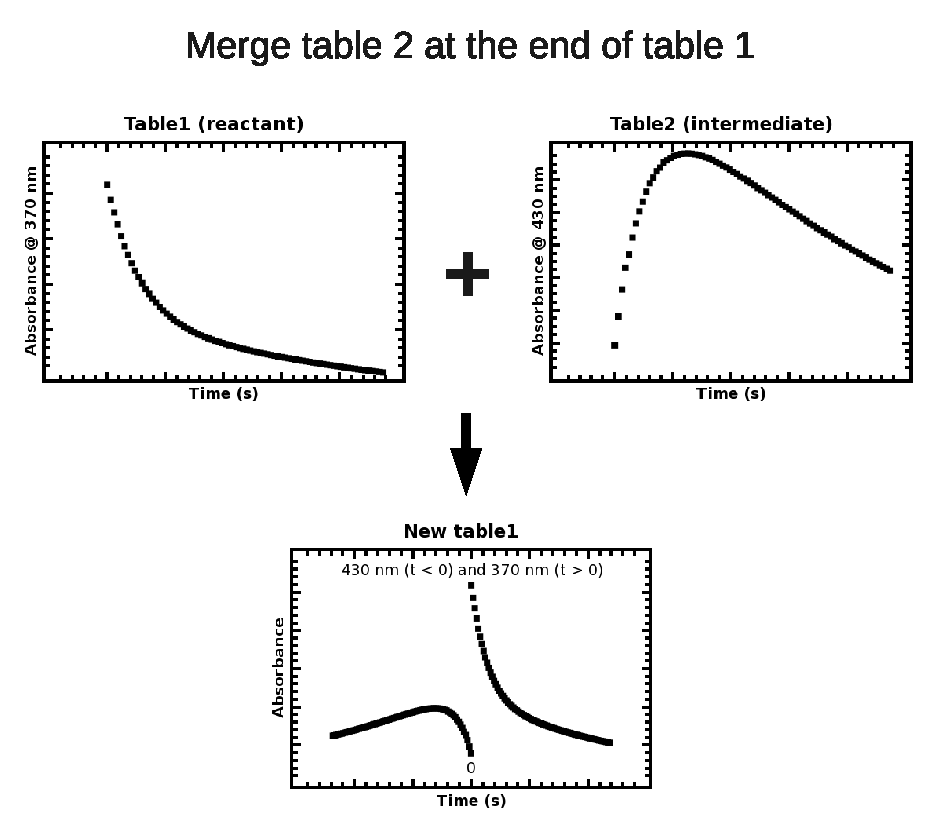
\includegraphics[scale=0.8]{merge}
\caption{Merging tables 1 and 2 in qtiplot.}
\label{merge}
\end{center}
\end{figure}

\section{Written laboratory report}

Follow the general instructions for written laboratory reports. In addition, include the requested data in the following section:\\

\noindent
\textit{Results.} This section should include the values and error estimates for $k_1$, $k_2$ and $k_3$. Your error analysis should be based on the error estimates given by the qtiplot program. Report also the $r^2$ value for your fit. There are no literature values available for this experiment.

\section{References}

\vspace{-1cm}

\bibliography{../../references}

\end{document}
